\chapter{图件总表}
\label{ch:figures}

本章按图位登记对象、坐标、来源和不能支持的句子。图位分为机制图、数学图、数据图和实施例图。基础部分为机制图 28 幅、数学图 16 幅、数据图 24 幅、实施例 8 幅。扩展面板 D25--D36 仍从同一日志取列，不新增科学主张。合计 88 个图号。分面板用 (a)(b)(c)，不另计图号。

已经画出的数据图是 D1、D6、D7、D10、D25，图放在第 \ref{ch:sim} 章，这里不再重复插入。其余数据图位没有对应日志，不绘制曲线。Q1--Q6 的证明几何放在第 \ref{ch:proof} 章。本章不把证明几何再画一遍，只登记每个图位能支持哪一句、不能支持哪一句。
\section{机制图}

机制图表达变量之间的依存。图中的箭来自已经写出的方程或模块合同。没有测量的边不标数值。

\subsection{M1 四个决策与信息赤字}
\paragraph{对象}
四个判断——能否停止、表面含水是否偏离、温度是否仍在散开、继续施加边界是否安全——各自对信息赤字 $\Delta\mathcal{I}$ 的贡献。

\paragraph{坐标与应读出的关系}
横轴是四个判断，纵轴是该判断的剩余熵减掉允许误判。柱高于零表示这个判断仍缺信息。四个柱可以同时为正，也可以只有停机为正。

\paragraph{与方程的对应}
赤字的定义在第 1 章：$\Delta\mathcal{I}=H(\phi(\vect{x})\mid\vect{y}_{0:t})-H_{\mathrm{tol}}$。$\phi$ 分别取冷点进度、表面含水、温度标准差和硬安全指示。四条柱不共享一个阈值。

\paragraph{来源}
机制图。它不读取 S1 日志。允许误判由动作切换的滞回带决定，本次没有用外部温度历程标定 $H_{\mathrm{tol}}$。

\paragraph{该图位允许支持的句子}
可以写：停机赤字与表面赤字是两个泛函，腔温采样只进入边界输入，不自动降低内部进度的熵。

\paragraph{该图位不能支持的句子}
不能把柱高写成某一菜谱还要几分钟。不能把四个判断合并成一个“熟度百分比”。

\subsection{M2 六步闭环与真值隔离}
\paragraph{对象}
真值生成、带噪采样、后验、安全投影、写回边界、用真值场评分，这六步的数据流，以及真值不得进入在线模块的切口。

\paragraph{坐标与应读出的关系}
六步沿环排列。切口画在第 2 步：在线模块的输入只有可安装通道。评分箭从真值场指向指标，不指向执行器。

\paragraph{与方程的对应}
完整性条件是第 1 章的六条。热阻更新若使用由真值温差构成的 $r_{\mathrm{proxy}}$，箭头就穿过了切口。

\paragraph{来源}
机制图，对照本次核的接口。核在“是否更接近参照”这一步读了真值温差，所以图上该箭要标成已发生的泄漏，而不是理想环。

\paragraph{该图位允许支持的句子}
可以写：本次方差下降必须和参照一起报告，因为参照不是传感器。

\paragraph{该图位不能支持的句子}
不能把画成闭环的箭头写成异构真值已经隔离。积分器是十六条控制体，不是带压力方程的多孔介质真值。

\subsection{M3 五层与唯一执行器接口}
\paragraph{对象}
物理场、决策状态、估计、解释、执行五层，以及只有执行层能写执行器。

\paragraph{坐标与应读出的关系}
五层自上而下。向下的箭只携带分布或分位数。唯一向上写回执行器的箭从安全投影出发。

\paragraph{与方程的对应}
模块合同在第 3 章：层间不传递对方的内部数组。品质模型的输出在进入执行器前被只依赖硬测量的不等式投影。

\paragraph{来源}
机制图。本次实现把积分、策略和评分放在同一次循环里，层间隔离没有落在目录边界上。

\paragraph{该图位允许支持的句子}
可以写：合同要求控制器读分位数；本次跟踪器交出的是 $(\hat T_c,\hat r,\mathrm{Var}(r))$ 三个标量。

\paragraph{该图位不能支持的句子}
不能把五层框图写成五个进程已经分开部署。

\subsection{M4 四个时间尺度的中断}
\paragraph{对象}
电气安全、热安全、信息探针、品质菜单四个时间尺度，以及快环打断慢环的方向。

\paragraph{坐标与应读出的关系}
横轴是时间尺度的量级：毫秒至秒、秒、数十秒、分钟。箭头只能从更快的环指向更慢的环，表示打断。

\paragraph{与方程的对应}
探针窗 40 s 位于信息尺度。品质菜单是 $900$、$1170$、$1530$ s。加热器时间常数约 $43$ s，与探针窗同一量级，所以探针期间加热器状态不能当成已达平衡。

\paragraph{来源}
机制图，常数来自附录的尺度算术，不是示波器记录。

\paragraph{该图位允许支持的句子}
可以写：停机后的低功率仍可能继续累积 $F$，评价必须用停机时刻的 $\alpha_m$。

\paragraph{该图位不能支持的句子}
不能把四个尺度写成已经由中断优先级的代码实现。本次模式整数只有品质、探针和保持。

\subsection{M5 模块合同只传递分布}
\paragraph{对象}
估计模块交给控制模块的对象是 $p(\vect{z}\mid\vect{y})$，不是一个点估计。

\paragraph{坐标与应读出的关系}
左侧是观测，中间是后验，右侧是机会约束使用的分位。点估计若出现，只能作为对照箭，并且标成合同之外。

\paragraph{与方程的对应}
决策充分性要求代价是 $\vect{z}$ 的 Lipschitz 函数，并且后验不确定度低于切换滞回。均值一个数不包含不确定度，因此不满足合同。

\paragraph{来源}
机制图。本次加热律用的是 $\hat T_c$ 加一条由 $\sqrt{\mathrm{Var}}$ 写成的裕量，裕量不是后验分位。

\paragraph{该图位允许支持的句子}
可以写：裕量 $\mu=6+10\sqrt{\mathrm{Var}(r)}\,(L/0.03)$ 是一个手写宽度，不是集合样本的经验分位。

\paragraph{该图位不能支持的句子}
不能写成控制器已经在读 32 个集合成员。没有这次运行。

\subsection{M6 三相与界面}
\paragraph{对象}
固相体积分数 $\varepsilon_s(S)$、液相 $\varepsilon_l$、气相 $\varepsilon_g$，以及食品与腔体的界面 $\Gamma$。

\paragraph{坐标与应读出的关系}
一个代表体元内三相之和为 1。界面一侧是食品未知量，另一侧是边界输入 $(T_\infty,Y_\infty,\vect{v}_\infty,\dot m_{\mathrm{st}},P_{\mathrm{heat}})$。

\paragraph{与方程的对应}
约束写在第 \ref{ch:physics} 章。$S$ 综合收缩、孔隙闭合与结壳，不是某一个分子机理的别名。

\paragraph{来源}
机制图。十六条控制体只有温度和含水两个场，没有独立的 $\varepsilon_g$ 和 $p_g$。

\paragraph{该图位允许支持的句子}
可以写：腔体状态是执行器，不是食品的隐藏状态。

\paragraph{该图位不能支持的句子}
不能把体元示意图写成孔隙尺度的弯月面已经被跟踪。

\subsection{M7 能量方程的四项}
\paragraph{对象}
导热、流体携带的显热、相变潜热、反应热，在能量方程右端的位置。

\paragraph{坐标与应读出的关系}
四项画成进入代表体元的箭。潜热的方向由蒸发或冷凝决定，不由模式名称决定。

\paragraph{与方程的对应}
连续形式是式 \eqref{eq:energy}。核把潜热收成 $q_{\mathrm{lat}}=18000\,u_{\mathrm{st}}(1-a_w)-9000\,(1-u_{\mathrm{st}})\max(a_w-0.35,0)\,u_{\mathrm{fan}}$，显热对流和反应热没有各自的场。

\paragraph{来源}
机制图。系数 18000 与 9000 是工程核的设定，不是由蒸汽表标定的体积源项。

\paragraph{该图位允许支持的句子}
可以写：核保留了冷凝放热、蒸发吸热的方向，没有保留式 \eqref{eq:phase} 对局部蒸汽压的依赖。

\paragraph{该图位不能支持的句子}
不能用 S1 的温度曲线核对式 \eqref{eq:energy} 的每一项，因为核没有 $\dot m_{\mathrm{phase}}$ 场。

\subsection{M8 潜热符号的切换}
\paragraph{对象}
冷凝与蒸发对 $q_{\mathrm{lat}}$ 符号的切换条件。

\paragraph{坐标与应读出的关系}
横轴是表面蒸汽压与饱和压之差，纵轴是界面潜热。正半轴为冷凝放热，负半轴为蒸发吸热。

\paragraph{与方程的对应}
规格中的切换由 $(p_v-p_{\mathrm{sat}})$ 的符号决定，见式 \eqref{eq:phase}。核中的切换由蒸汽指令 $u_{\mathrm{st}}$ 是否为 1 决定，活度只调制幅度。

\paragraph{来源}
机制图。两条切换规则要分两层画，不能画成同一条折线。

\paragraph{该图位允许支持的句子}
可以写：蒸制时核令蒸汽指令为 1，潜热取正号的第一项；烤制时第一项为零，第二项为吸热。

\paragraph{该图位不能支持的句子}
不能把“当前模式叫做蒸”写成 $p_v>p_{\mathrm{sat}}$ 已经成立。核没有蒸汽压未知量。

\subsection{M9 四条反应进度}
\paragraph{对象}
蛋白质变性 $\alpha_p$、淀粉糊化 $\alpha_g$、美拉德褐变 $\alpha_b$、致死当量 $\alpha_m$ 对温度和水分的开关差异。

\paragraph{坐标与应读出的关系}
四条进度对同一条温度史的响应。纵轴为 $[0,1]$。表面高温干燥时 $\alpha_b$ 上升，冷点上的 $\alpha_m$ 可以仍低。

\paragraph{与方程的对应}
速率结构是式 \eqref{eq:kinetics}。核里的褐变是 $\Delta t\cdot 2\times 10^{-4}\max(T_0-110,0)\max(0.55-m_0,0)$，不是该式的 $A_i$ 与 $E_{a,i}$。$\alpha_m=1-\mathrm{e}^{-F/2}$，$F$ 只在冷点上积分。

\paragraph{来源}
机制图。活化能扫描没有做。

\paragraph{该图位允许支持的句子}
可以写：停机不能定义成中心温度超过某一个数，因为同一条中心温度可以对应不同的表面褐变。

\paragraph{该图位不能支持的句子}
不能把 $2\times 10^{-4}$ 写成美拉德反应的频率因子。$\alpha_m$ 不含微生物的初始数量。

\subsection{M10 结壳增大内部热阻}
\paragraph{对象}
表面结壳 $S$ 增大 $R_{\mathrm{int}}$、降低渗透率，使冷点进度落后于表面褐变。

\paragraph{坐标与应读出的关系}
一条正反馈：表面变干 $\to S$ 上升 $\to$ 内部热阻上升 $\to$ 冷点更慢 $\to$ 表面继续变干。

\paragraph{与方程的对应}
规格是式 \eqref{eq:structure} 与式 \eqref{eq:shrink}。核里 $S$ 只在表面含水低于 $0.45$ 时以 $1.5\times 10^{-4}\,\mathrm{s}^{-1}$ 增长，并且只进入 $r_{\mathrm{proxy}}$，不改导热场。

\paragraph{来源}
机制图。路径 C 在核里没有闭合。

\paragraph{该图位允许支持的句子}
可以写：结壳变量影响的是“更新是否更接近参照”，不是网格上的 $k$。

\paragraph{该图位不能支持的句子}
不能把这条反馈画成 S1 已经测到壳层热阻随时间的曲线。没有 $R_{\mathrm{int}}(t)$ 的测量列。

\subsection{M11 全场到决策状态}
\paragraph{对象}
映射 $\Phi:\vect{X}\mapsto\vect{z}$。全场含温度、气相压力、液相分数、蒸汽质量分数、四条进度和结构。决策状态是九个泛函。

\paragraph{坐标与应读出的关系}
左侧是场，右侧是式 \eqref{eq:z} 的九个分量。没有箭指向的场分量不进入控制器。

\paragraph{与方程的对应}
决策充分性：若代价与约束都是 $\vect{z}$ 的 Lipschitz 函数，且后验不确定度低于滞回带，则细化网格不改变已投影的安全动作。

\paragraph{来源}
机制图。日志给出冷点温度、表面温度、平均含水和 $\alpha_m$。$\sigma_T$、表面液相、表面褐变、表面结壳和累计失重没有全部进入停机规则。

\paragraph{该图位允许支持的句子}
可以写：在线模型只要在 $\vect{z}$ 上可比，允许是径向多孔介质、两节点或神经算子。后两者里，两节点只用于辨识，神经算子没有训练。

\paragraph{该图位不能支持的句子}
不能用该命题裁剪传感器。Lipschitz 常数没有标定。

\subsection{M12 GAB 形状差异}
\paragraph{对象}
吸附等温线随 $X_m$、$C$、$K$ 与温度改变的方向。肉类没有清洁行，不画肉类数据点。

\paragraph{坐标与应读出的关系}
横轴活度，纵轴干基含水。至少两条曲线：土豆吸附 $30^\circ\mathrm{C}$ 与 $60^\circ\mathrm{C}$。参数来自记录 c074 与 c076。

\paragraph{与方程的对应}
式 \eqref{eq:gab}。c074 在活度 $0.2$、$0.4$、$0.6$、$0.8$ 给出含水约 $0.053$、$0.080$、$0.118$、$0.204$。c076 给出约 $0.023$、$0.038$、$0.056$、$0.084$。

\paragraph{来源}
数据来自 \cite{sorption2026} 的清洁子集，不是本次蒸烤实验。温度只到 $60^\circ\mathrm{C}$。

\paragraph{该图位允许支持的句子}
可以写：同一活度下，测定温度升高时含水下降。

\paragraph{该图位不能支持的句子}
不能把曲线外推到烤制表面。不能把土豆参数标成肉糜的测定。不能在图上补肉类点。

\subsection{M13 各向异性与脂肪夹层}
\paragraph{对象}
纤维方向导热 $k_\parallel$、$k_\perp$ 与脂肪夹层在冷点路径上的位置。

\paragraph{坐标与应读出的关系}
一张二维截面。脂肪层不必放在几何中心。冷点可以落在低导热层的背侧。

\paragraph{与方程的对应}
式 \eqref{eq:aniso} 与并联热阻 $R_{\mathrm{fat}}=L_{\mathrm{fat}}/(k_{\mathrm{fat}}A)$。核的非均质档 2 只把下标 5 的控制体导热乘 $0.45$。额外热阻约占十六条串联热阻的 $7.6\%$，因为只有一个控制体变厚热阻。

\paragraph{来源}
机制图。T2 的二维脂肪几何没有运行。

\paragraph{该图位允许支持的句子}
可以写：档 2 是一块低导热夹层，不是连续脂肪几何，也没有纤维方向。

\paragraph{该图位不能支持的句子}
不能把下标 5 的位置写成冷点已经离开中心的测量。冷点在核里是十六个体的最低温度，不输出空间坐标。

\subsection{M14 收缩与渗透率}
\paragraph{对象}
厚度 $L$ 随蛋白进度下降，渗透率 $K$ 随厚度和气相分数一起变。

\paragraph{坐标与应读出的关系}
横轴是 $\alpha_p$ 或含水，左轴是 $L/L_0$，右轴是 $K/K_0$。两条曲线都是规格中的单调关系，不画未运行的轨迹。

\paragraph{与方程的对应}
式 \eqref{eq:shrink}：$\dot L=-\beta_s L_0\dot\alpha_p$，$K=K_0(L/L_0)^{n_K}\varepsilon_g^{n_\varepsilon}$。核内一条轨迹的厚度是常数。

\paragraph{来源}
机制图。$\beta_s$、$n_K$、$n_\varepsilon$ 没有在 S1 里扫描。

\paragraph{该图位允许支持的句子}
可以写：厚度固定时，Fourier 数只随时间和扩散率变，不随收缩变。

\paragraph{该图位不能支持的句子}
不能把菜单时间 $900$、$1170$、$1530$ s 解释成已经计入了收缩。

\subsection{M15 角系数}
\paragraph{对象}
加热管、腔壁、食品表面之间的角系数 $F_{h,s}$ 与 $F_{w,s}$。

\paragraph{坐标与应读出的关系}
三个表面。箭的粗细表示角系数的数量级，本次没有测量值，因此只标符号，不标数值。

\paragraph{与方程的对应}
辐射边界 $q_{\mathrm{rad}}=F_{h,s}\epsilon_s\sigma(T_h^4-T_s^4)+F_{w,s}\epsilon_s\sigma(T_w^4-T_s^4)$。核把辐射吸收进 $7000\,u$ 和 $T_\infty=90+95\,u$，没有 $T^4$。

\paragraph{来源}
机制图。角系数不是 S1 的因子。

\paragraph{该图位允许支持的句子}
可以写：热像里的反射项与 $F_{h,s}T_h^4$ 是同一几何量。核里没有这一项。

\paragraph{该图位不能支持的句子}
不能用核的温度曲线反推发射率或角系数。

\subsection{M16 红外亮度}
\paragraph{对象}
热像亮度中的发射项与反射项。

\paragraph{坐标与应读出的关系}
表面。离开表面的辐射等于 $\epsilon T_s^4$ 加上 $(1-\epsilon)$ 乘来自加热管和腔壁的照射。

\paragraph{与方程的对应}
观测算子式 \eqref{eq:ir}。发射率与结壳绑定，作为慢变参数。本次战役没有热像通道。

\paragraph{来源}
机制图。没有红外图像日志。

\paragraph{该图位允许支持的句子}
可以写：表面温度的带噪读数是接触式通道的替代，不是亮度反演。噪声幅度 $0.4^\circ\mathrm{C}$ 是设定，不是热像仪的 NETD。

\paragraph{该图位不能支持的句子}
不能把 D1 的表面温度写成红外反演的结果。

\subsection{M17 冷点偏离几何中心}
\paragraph{对象}
两种使最低温度离开厚度中点的边界：初始温度沿厚度倾斜，以及一个低导热控制体。

\paragraph{坐标与应读出的关系}
横轴是控制体下标 $0$ 到 $15$。两条温度折线只说明机制，不充当某次终止时刻的云图。

\paragraph{与方程的对应}
档 1 把初始温度加上从 $-4^\circ\mathrm{C}$ 到 $+4^\circ\mathrm{C}$ 的线性倾斜。档 2 把下标 5 的导热改为 $0.45k$。冷点定义为十六个体的最低温度，不记录其下标。

\paragraph{来源}
机制图。\cite{feyissa2013} 给出冷点可以偏离几何中心这一现象；本文不继承该文的网格和肉块物性。

\paragraph{该图位允许支持的句子}
可以写：最低温度不必是下标 15。核没有把该下标写入日志。

\paragraph{该图位不能支持的句子}
不能把示意折线读成 T2 的终止温度分布。D5 要求的空间曲线没有日志。

\subsection{M18 P4 的两段时序}
\paragraph{对象}
探针库元素 P4：先蒸汽、后气流。两段改变的输入方向不同。

\paragraph{坐标与应读出的关系}
横轴时间。第一段蒸汽指令为 1、风机维持；第二段蒸汽为 0、风机升高。规格上限短于已运行的 40 s 窗。

\paragraph{与方程的对应}
命题 \ref{prop:pulse}。已运行窗是 $[150,190)$ s：170 s 之前蒸汽为 1，其后风机为 1.3。这是固定窗，不是库上的一次优化。

\paragraph{来源}
机制图，与第 \ref{ch:ati} 章的时序一致。断言里两段滞后 $40.846$，单段 $38.912$，差 $1.934$，用的是 $+1$ 准则。

\paragraph{该图位允许支持的句子}
可以写：第二段必须增加一个不与 $T_\infty$ 共线的输入方向，否则内外热阻的灵敏度列相关。

\paragraph{该图位不能支持的句子}
不能把固定窗写成 $\arg\max G(a)-\lambda C(a)$ 的解。P0、P1、P2 没有日志。

\subsection{M19 表面时间常数与冷点窗口}
\paragraph{对象}
表面响应在短窗内抬升，冷点响应仍是 $O(\tau/\tau_2)$。

\paragraph{坐标与应读出的关系}
横轴时间，纵轴温度增量。一条快曲线、一条慢曲线。窗的右端落在慢曲线尚未离开初值的位置。

\paragraph{与方程的对应}
命题 \ref{prop:budget}：$|\Delta T_2|\le (\tau/\tau_2)\Delta T_s$。断言常数 $\tau_2=30$ s、$\tau=3$ s、$\Delta T_s=12$ K，上界 $1.2$ K，离散积分 $1.143$ K。战役窗是 40 s，不是这组常数。

\paragraph{来源}
机制图加断言算术。种子 7 在 152 s 至 192 s 的冷点增量约 $0.04$ K，表面增量约 $8.5$ K。这是一条轨迹。

\paragraph{该图位允许支持的句子}
可以写：40 s、30 mm 的 Fourier 数是 $8.9\times 10^{-3}$，边界变化还没有穿过该厚度。

\paragraph{该图位不能支持的句子}
不能把 $1.143$ K 写成 S1 探针的冷点增量。不能把“几乎不推动”推广到任意时长。

\subsection{M20 信息项随赤字开闭}
\paragraph{对象}
对偶目标里 $\lambda_I$ 在赤字为正时打开，赤字低于零且安全分位已通过时关闭。

\paragraph{坐标与应读出的关系}
横轴是 $\Delta\mathcal{I}$，纵轴是信息项权重。零点左侧权重为零。

\paragraph{与方程的对应}
式 \eqref{eq:dual}。关闭之后最优解退回纯品质控制。

\paragraph{来源}
机制图。本次对偶策略在方差下降之后仍使用带 $\sqrt{\mathrm{Var}}$ 的裕量，信息项没有被关掉。

\paragraph{该图位允许支持的句子}
可以写：$\lambda_I=0$ 的极限没有作为单独策略出现在日志里。

\paragraph{该图位不能支持的句子}
不能把能量中位数从 1655 到 1730 的差别写成 $\lambda_E$ 已经标定。

\subsection{M21 父节点固定的结构图}
\paragraph{对象}
结构方程的父节点由机理指定。一次烹饪的短序列只允许调整函数参数和事先声明的可选边。

\paragraph{坐标与应读出的关系}
有向无环图。子节点与父节点的对照表与第 \ref{ch:causal} 章一致：界面蒸汽压、表面温度、内部温度、表面含水、三条进度、结壳。

\paragraph{与方程的对应}
式 \eqref{eq:scm}：$Z_i=f_i(\mathrm{Pa}_i,U_i)$。

\paragraph{来源}
机制图。父节点不由独立性检验从短序列里重新发现。

\paragraph{该图位允许支持的句子}
可以写：能量守恒不是从数据里学出来的边。

\paragraph{该图位不能支持的句子}
不能把图上的箭头写成干预效应的数值已经估计出来。

\subsection{M22 三条路径的分叉与汇合}
\paragraph{对象}
路径 A：蒸汽经潜热进入冷点。路径 B：蒸汽经表面含水进入褐变和失重。路径 C：结壳经内部热阻再进入冷点。A 与 C 在冷点汇合，B 停在表面品质。

\paragraph{坐标与应读出的关系}
一个分叉点在界面蒸汽，两个汇合点分别在冷点和表面品质。每条边标符号，不标尚未计算的增益数值。

\paragraph{与方程的对应}
式 \eqref{eq:path}。符号由父节点的物理方向决定。解释只在符号沿后验样本保持不变时给出。

\paragraph{来源}
机制图。核没有沿三条路径分别积分。路径 C 不改导热场。

\paragraph{该图位允许支持的句子}
可以写：同一次蒸汽动作可以同时推动冷点和损伤表面，两条边的符号不必相同。

\paragraph{该图位不能支持的句子}
不能把 S1 的策略差写成 $\mathrm{do}$ 算子的效应。策略差里混有停机规则。

\subsection{M23 预测、干预、反事实}
\paragraph{对象}
三个计算：条件预测、干预、反事实。三者的输入图不同。

\paragraph{坐标与应读出的关系}
三列。预测保留全部箭。干预切断指向被操纵变量的策略箭。反事实还要保留同一噪声实现。

\paragraph{与方程的对应}
语义继承 \cite{pearl2009}。本文的操纵变量是边界蒸汽、风机和加热，不是食品内部的进度。

\paragraph{来源}
机制图。三个计算都没有在日志上数值执行。

\paragraph{该图位允许支持的句子}
可以写：只做条件相关会把操作者习惯打开蒸汽的那些样本当成蒸汽的效应。

\paragraph{该图位不能支持的句子}
不能报告干预后的冷点位移。没有该列。

\subsection{M24 物理项、有界残差、回退}
\paragraph{对象}
在线模型由物理项、有界残差和越界回退三部分组成。残差超过 $r_{\max}$ 时丢弃残差，退回物理项。

\paragraph{坐标与应读出的关系}
横轴是残差范数，纵轴是是否写回。阈值右侧是回退区。

\paragraph{与方程的对应}
式 \eqref{eq:op} 与式 \eqref{eq:bnp}。回退之后控制器看到的是物理模型的 $\vect{z}$，不是残差网络的输出。

\paragraph{来源}
机制图。残差网络没有训练，没有 $r_{\max}$ 的数值，没有回退次数。

\paragraph{该图位允许支持的句子}
可以写：未训练时，在线更新只剩下标量热阻及其方差。

\paragraph{该图位不能支持的句子}
不能把 D18 画成回退次数曲线。该图位没有日志。

\subsection{M25 类别先验的精度加权}
\paragraph{对象}
一次烹饪的似然与类别先验按精度加权。似然与先验冲突且没有标记时，拒绝写回类别库。

\paragraph{坐标与应读出的关系}
两个高斯的精度 $1/\sigma^2$ 决定后验均值的位置。拒绝写回画成一条不进入类别库的箭。

\paragraph{与方程的对应}
式 \eqref{eq:hier}。单次轨迹不覆盖整个类别。

\paragraph{来源}
机制图。本次没有类别库的写回操作。所有行的扩充标记为假。

\paragraph{该图位允许支持的句子}
可以写：食材类别只改先验和终端目标，不改 $\vect{z}$ 的分量定义。

\paragraph{该图位不能支持的句子}
不能把三种食材的中位数几乎相同写成类别库已经更新。原因是高含水段活度饱和，见第 \ref{ch:data} 章。

\subsection{M26 候选执行量到安全集的投影}
\paragraph{对象}
品质模型给出的加热请求先进入安全集，再写执行器。安全集由硬测量定义，不随后验变形。

\paragraph{坐标与应读出的关系}
横轴是请求，纵轴是投影后的指令。安全集是一条不依赖后验的截断。

\paragraph{与方程的对应}
式 \eqref{eq:cbf}。命题 \ref{prop:shield}：加热器温度超过阈值时，不同后验得到同一投影。断言函数在 $210^\circ\mathrm{C}$ 把请求剪到 $0.25$。核的削减从 $230^\circ\mathrm{C}$ 开始，平衡点是 $196.5^\circ\mathrm{C}$。

\paragraph{来源}
机制图加两段代码的常数。两段都通过“不读后验”这一句，阈值不同。

\paragraph{该图位允许支持的句子}
可以写：本次战役的加热器轨迹不进入削减区，投影没有改变指令。

\paragraph{该图位不能支持的句子}
不能把断言通过写成 $230^\circ\mathrm{C}$ 削减已经在 S1 里动作。

\subsection{M27 五级降级的方向}
\paragraph{对象}
降级只向更少依赖估计的方向：全功能、尾部约束并关闭解释、物理降阶并保留探针、宽区间保温、硬件断电。

\paragraph{坐标与应读出的关系}
五级从左到右。箭头单向。没有从硬件断电回到全功能的数据箭。

\paragraph{与方程的对应}
第 \ref{ch:safe} 章的状态机规格。级别由通道是否有效和屏障是否接近决定，不由剩余时间点决定。

\paragraph{来源}
机制图。本次模式整数是品质、探针、保持。保持是停机后的低功率，不是“通道失效”那一级。没有停留时间日志。

\paragraph{该图位允许支持的句子}
可以写：界面若输出剩余时间，必须输出区间；没有区间时这一级的页面不应出现单点分钟数。

\paragraph{该图位不能支持的句子}
不能报告各级停留时间。D24 没有日志。

\subsection{M28 两条测量链}
\paragraph{对象}
品质测量链与硬测量链分开。硬链包含剩余电流、加热管壳体温度、腔压、门封温度、门开关。品质链包含表面温度、质量和湿度。

\paragraph{坐标与应读出的关系}
两条链在投影之前不相交。硬链直接进入屏障不等式。

\paragraph{与方程的对应}
第 \ref{ch:safe} 章。硬链的读数不进入品质网络的特征。

\paragraph{来源}
机制图。本次步进里与安全有关的状态只有加热器温度。空烧、剩余电流、腔压和门没有变量。

\paragraph{该图位允许支持的句子}
可以写：干烧保护若只依赖水位传感器，传感器粘滞时要由管温的温升速率接上。这一路没有采样。

\paragraph{该图位不能支持的句子}
不能把加热器 ODE 的存在写成干烧保护已经检验。S2 没有注入空烧。

\section{数学图}

数学图表达证明或病态性的几何。Q1--Q6 只含命题中的关系。需要数值秩而尚未计算的图位只保留坐标，不画示意曲线。

\subsection{Q1 平衡点处灵敏度列消失}
\paragraph{对象}
内部热阻变化时，平衡温度保持为 $T_\infty$ 的一条水平线。

\paragraph{坐标与应读出的关系}
横轴 $R_{\mathrm{int}}$，纵轴温度。水平线位于 $T_\infty$。不画离开平衡之后的瞬态。

\paragraph{与方程的对应}
命题 \ref{prop:steady}。无相变且质量流为零时，$T_1=T_2=T_\infty$，$(R_{\mathrm{int}},C_1,C_2)$ 只作为除数出现。

\paragraph{来源}
证明的几何。断言对 $R\in\{1,3,6\}$ 的平衡温差极差为 0。

\paragraph{该图位允许支持的句子}
可以写：恒温段再密的腔温采样也不更新内部热阻。

\paragraph{该图位不能支持的句子}
不能把水平线读成 S1 的散点。不能把极差为 0 写成离开平衡后的灵敏度也是 0。

\subsection{Q2 两段脉冲后的两列灵敏度}
\paragraph{对象}
仅改变环境温度时输入矩阵是单列；潜热在两节点方程里与之共线。加一段气流之后，内外热阻的灵敏度列线性无关。

\paragraph{坐标与应读出的关系}
平面上的两个向量。第一段之后两列共线，第二段之后张成面积不为零。

\paragraph{与方程的对应}
命题 \ref{prop:pulse}。断言比较的是滞后而不是行列式：$40.846>38.912+1$。相对 $1.15$ 倍不成立，因为比值约 $1.050$。

\paragraph{来源}
证明的几何加断言里的两个滞后数。滞后来自两节点断言函数，不是 S1 的热阻误差。

\paragraph{该图位允许支持的句子}
可以写：第二段要贡献的是一个新方向，不是把同一列再放大一个固定百分比。

\paragraph{该图位不能支持的句子}
不能把 $1.934$ 的滞后差写成 S1 里信息增益的奈特数。

\subsection{Q3 冷点增量上界}
\paragraph{对象}
短窗内冷点增量不超过窗长与内部时间常数之比乘表面增量。

\paragraph{坐标与应读出的关系}
横轴 $\tau/\tau_2$，纵轴 $|\Delta T_2|/\Delta T_s$。上界是过原点的直线。断言的一个点落在直线下方。

\paragraph{与方程的对应}
命题 \ref{prop:budget}。点的坐标是 $3/30=0.1$ 与 $1.143/12=0.0953$。

\paragraph{来源}
证明的几何。时间常数不是 40 s 的战役窗。

\paragraph{该图位允许支持的句子}
可以写：上界成立只说明在这组常数下离散积分没有越过直线。

\paragraph{该图位不能支持的句子}
不能把该点读成种子 7 的冷点增量。种子 7 的增量约 $0.04$ K，用的是另一组时间。

\subsection{Q4 分位、阈值与滞回}
\paragraph{对象}
停止阈值、不确定度带和滞回宽度三者的位置。滞回防止估计在阈值附近来回切换。

\paragraph{坐标与应读出的关系}
横轴是估计冷点。阈值在 $75+\mu$。滞回带画在阈值两侧。分位区间若同时盖住“未达”和“已过”，停机权利取消。

\paragraph{与方程的对应}
命题 \ref{prop:invalid}。核的实现是：方差仍大于 $0.45$ 且厚度大于 $40$ mm 时否决停止。没有分位区间。

\paragraph{来源}
证明几何与一条退化规则。Q4 不把滞回常数画进 Q5 的可行域。

\paragraph{该图位允许支持的句子}
可以写：否决的是停止时刻，不是加热请求。请求可以继续。

\paragraph{该图位不能支持的句子}
不能把 $0.45$ 写成 Fisher 矩阵的最小特征值。没有特征值。

\subsection{Q5 可行域不随后验变形}
\paragraph{对象}
安全集的边界由加热器温度定义。后验从 $0.1$ 变到 $0.9$ 时，同一请求得到同一投影。

\paragraph{坐标与应读出的关系}
请求—指令平面上的一条截断。两个后验点重合。

\paragraph{与方程的对应}
命题 \ref{prop:shield}。断言：加热器 $230^\circ\mathrm{C}$ 时请求 $1$ 被剪到 $0.25$，且与后验无关；加热器 $100^\circ\mathrm{C}$ 时不剪。

\paragraph{来源}
证明的几何。核的削减公式起点是 $230^\circ\mathrm{C}$，平衡点 $196.5^\circ\mathrm{C}$ 使该公式在战役里没有工作点。

\paragraph{该图位允许支持的句子}
可以写：两条规则说明同一件事的两个层次，阈值并不相同。

\paragraph{该图位不能支持的句子}
不能把重合的两个点读成 S1 里投影改变了能量中位数。

\subsection{Q6 链式法则的三支}
\paragraph{对象}
蒸汽对冷点和表面品质的导数拆成路径 A、B、C 三项。

\paragraph{坐标与应读出的关系}
三条并行的乘积链。每一支标父节点的偏导符号。数值增益留空。

\paragraph{与方程的对应}
命题 \ref{prop:path} 与式 \eqref{eq:path}。解释条件是符号沿后验样本不变。

\paragraph{来源}
证明的几何。核没有对三条路径分别积分。

\paragraph{该图位允许支持的句子}
可以写：路径 B 的符号可以与路径 A 相反，所以加大蒸汽不必同时改善冷点和表面。

\paragraph{该图位不能支持的句子}
不能在链上填 S1 的策略差。策略差不是路径增益。

\subsection{Q7 傅里叶、毕渥与柯斯勒数的区域}
\paragraph{对象}
内部导热、外部对流和潜热相对显热，三个无量纲数把过程分成不同区域。

\paragraph{坐标与应读出的关系}
横轴 Fourier 数，纵轴 Biot 数。Ko 用区域标注而不是第三根轴的假数据。

\paragraph{与方程的对应}
定义 $\mathrm{Fo}=\alpha t/L^2$，$\mathrm{Bi}=hL/k$，$\mathrm{Ko}=\Delta h\,\varepsilon_{l0}\rho_l/((\rho c)\Delta T)$。已算出的点只有附录里的尺度：40 s、30 mm 的 Fo 为 $8.9\times 10^{-3}$；风机 $0.4$ 时 15、30、50 mm 的 Bi 为 $0.75$、$1.5$、$2.5$。

\paragraph{来源}
尺度算术，扩散率是核的设定值 $2.0\times 10^{-7}\,\mathrm{m}^2/\mathrm{s}$。

\paragraph{该图位允许支持的句子}
可以写：三档厚度在探针窗内 Fo 都远小于 1。Bi 与 1 同量级，表面温度不能代替冷点。

\paragraph{该图位不能支持的句子}
不能把这几个点连成区域边界的实验曲线。Ko 没有用轨迹积分出来。

\subsection{Q8 逆热传导的误差放大}
\paragraph{对象}
表面高频误差传到冷点时的放大倍数随频率和厚度增加。

\paragraph{坐标与应读出的关系}
横轴频率，纵轴放大倍数，一族曲线以厚度为参数。图位先给出坐标。数值曲线留待逆问题计算完成。

\paragraph{与方程的对应}
放大的结构继承 \cite{ozisik2000}。本文不继承某一热像仪的标称精度。

\paragraph{来源}
坐标图位。没有数值秩，不绘制示意曲线充当结果。

\paragraph{该图位允许支持的句子}
可以写：厚度增大使同一频率的误差更难反演，这是被动观测有上限的原因。

\paragraph{该图位不能支持的句子}
不能读取图上的分贝数。分贝数没有计算。

\subsection{Q9 可观测矩阵的秩随热阻比恶化}
\paragraph{对象}
内部热阻相对外部热阻增大时，表面观测对冷点的灵敏度下降。

\paragraph{坐标与应读出的关系}
横轴 $R_{\mathrm{int}}/R_{\mathrm{ext}}$，纵轴可观测矩阵的最小奇异值。坐标先给出。奇异值曲线未计算。

\paragraph{与方程的对应}
两节点线性化后的可观测矩阵。平衡点上参数灵敏度已经由命题 \ref{prop:steady} 为零，这里的秩是离开平衡之后的状态可观测性。

\paragraph{来源}
坐标图位。没有数值秩。

\paragraph{该图位允许支持的句子}
可以写：状态可观测与参数可辨识不是同一件事。平衡温度对内部热阻的导数为零，并不表示两个温度节点在瞬态中不可区分。

\paragraph{该图位不能支持的句子}
不能把某条下降曲线读成已经算出的奇异值。

\subsection{Q10 湿度饱和段的信息量}
\paragraph{对象}
湿度读数接近饱和时，该通道对方差的贡献下降。

\paragraph{坐标与应读出的关系}
横轴是相对湿度或活度，纵轴是该通道的 Fisher 信息。饱和点取读数 $0.98$。

\paragraph{与方程的对应}
规格：读数超过 $0.98$ 时增大对应的观测方差。核的含水噪声是常数 $0.004$，没有这条规则。

\paragraph{来源}
坐标图位。S1 初含水上核的活度已经饱和到 $0.99$ 以上，但那是模型输出，不是湿度传感器的 Fisher 信息。

\paragraph{该图位允许支持的句子}
可以写：高含水段三个原型的活度几乎相同，食材交叉表重合与此一致。

\paragraph{该图位不能支持的句子}
不能把活度饱和写成湿度通道的信息量已经按 $0.98$ 规则下降。规则没有进入步进。

\subsection{Q11 探针库上的比较结构}
\paragraph{对象}
库中元素按 $G(a)-\lambda C(a)$ 比较，而不是按连续波形优化。

\paragraph{坐标与应读出的关系}
五个离散点 P0 至 P4。纵轴是信息增益减损伤。没有点的数值。

\paragraph{与方程的对应}
式 \eqref{eq:astar}。已运行的只有固定窗，对应库中的一个元素，且没有向前滚动。

\paragraph{来源}
坐标图位。五个元素的 $G$ 与 $C$ 都没有日志。

\paragraph{该图位允许支持的句子}
可以写：家电执行器只有有限探针库，连续最优波形不在可实施集合里。

\paragraph{该图位不能支持的句子}
不能把固定窗画成五个点中的最高点。没有比较。

\subsection{Q12 干预切断策略边}
\paragraph{对象}
条件相关保留“操作者在什么情况下开蒸汽”的边；干预把这条边切断，只保留蒸汽到食品状态的边。

\paragraph{坐标与应读出的关系}
两张图。右图上策略节点到蒸汽节点的箭被切断。

\paragraph{与方程的对应}
第 \ref{ch:causal} 章对预测、干预、反事实的区分。

\paragraph{来源}
机制化的数学图。没有在日志上执行 $\mathrm{do}$。

\paragraph{该图位允许支持的句子}
可以写：四条策略的 $e_\alpha$ 差别不是干预效应，因为策略同时改变了停机规则。

\paragraph{该图位不能支持的句子}
不能把 D10 的四个分布读成四次干预。

\subsection{Q13 残差界与回退}
\paragraph{对象}
残差范数超过 $r_{\max}$ 时，更新被丢弃。

\paragraph{坐标与应读出的关系}
横轴残差，纵轴写回指示。阈值是一条竖线。竖线的横坐标未标定。

\paragraph{与方程的对应}
式 \eqref{eq:bnp}。

\paragraph{来源}
坐标图位。没有残差网络，没有回退计数。

\paragraph{该图位允许支持的句子}
可以写：回退之后控制器使用的是物理项给出的决策状态。

\paragraph{该图位不能支持的句子}
不能读取回退次数。D18 没有日志。

\subsection{Q14 机会约束与尾部硬约束}
\paragraph{对象}
机会约束允许决策状态的分位越过一条软边界的概率不超过 $\varepsilon$。硬约束由屏障定义，不允许越界。

\paragraph{坐标与应读出的关系}
两个集合。硬安全集包含在更宽的机会约束可行集之内，或二者相交。包含关系画成规格，不画未求解的轨迹。

\paragraph{与方程的对应}
式 \eqref{eq:mpc} 与式 \eqref{eq:cbf}。CasADi 没有被调用。

\paragraph{来源}
数学图。没有求解器的可行域采样。

\paragraph{该图位允许支持的句子}
可以写：硬约束不读后验，机会约束读分位。本次加热律两者都没有求解。

\paragraph{该图位不能支持的句子}
不能把饱和线性加热律的输出点画进这个包含关系里充当最优解。

\subsection{Q15 预测时域与控制时域}
\paragraph{对象}
预测时域长于控制时域。控制时域之后的输入按终端策略保持，不逐拍自由。

\paragraph{坐标与应读出的关系}
横轴未来时间。控制时域 $N_c$ 短于预测时域 $N_p$。两者的拍数未标定。

\paragraph{与方程的对应}
预测控制的标准时域拆分，继承 \cite{rawlings2017}。本文不继承某一个求解器的默认拍数。

\paragraph{来源}
坐标图位。没有时域参数，因为求解器没有运行。

\paragraph{该图位允许支持的句子}
可以写：探针若进入预测控制，只能作为控制时域里的一段固定输入。

\paragraph{该图位不能支持的句子}
不能读取 $N_p$ 与 $N_c$ 的比值。

\subsection{Q16 真值与估计的数据隔离}
\paragraph{对象}
真值模型 T 与在线模型 E 不共享参数内存。评分只在 T 的场上计算。

\paragraph{坐标与应读出的关系}
两块内存。从 T 到 E 的箭只通过带噪观测。任何参数直连都标成隔离失败。

\paragraph{与方程的对应}
第 \ref{ch:sim} 章的双模型原则。

\paragraph{来源}
数学图，对照本次接口。热阻更新的参照使用真值温差，图上这条箭要标成泄漏。

\paragraph{该图位允许支持的句子}
可以写：同构自检不进入主表。本次没有异构配对。

\paragraph{该图位不能支持的句子}
不能把十六条控制体的自洽残差写成感知误差。

\section{数据图}

数据图只使用第 \ref{ch:sim} 章日志中的列。没有对应日志的图位保留坐标，不绘制曲线。D10 是主图。能量等次要指标不在 D10 缺席时单独作为结论。同构结果不进入摘要句。

D1--D24 是基础数据图。D25--D36 是同一日志的扩展面板，编号连续，不另起一套科学主张。

\subsection{D1 表面、冷点与估计}
\paragraph{对象}
一条轨迹上的表面温度、冷点温度和估计冷点。

\paragraph{坐标与应读出的关系}
横轴时间，纵轴温度。三条曲线。真值冷点与估计冷点的差是跟踪误差，不是分位带。

\paragraph{与方程的对应}
种子 7、肉糜、30 mm、对偶。$t=0$ 表面约 $11.4^\circ\mathrm{C}$，冷点 $8.0^\circ\mathrm{C}$，估计约 $-7.9^\circ\mathrm{C}$。负的估计是上限 $y_T-16$ K 的结果，不是传感器读到零下。

\paragraph{来源}
战役轨迹文件。记录间隔 8 s。它不在 4860 的初温格子里。

\paragraph{该图位允许支持的句子}
可以写：1200 s 时估计可以高于冷点，所以上限不是下置信界。

\paragraph{该图位不能支持的句子}
不能把这一条写成中位数。不能写成热像反演或物理实验。

\subsection{D2 液相分数}
\paragraph{对象}
表面液相分数与平均液相分数随时间的变化，并对照蒸、烤、组合。

\paragraph{坐标与应读出的关系}
横轴时间，纵轴液相分数。规格要求三条模式曲线。

\paragraph{与方程的对应}
核有平均含水列，没有把蒸、烤、组合拆成三套边界后的对照。

\paragraph{来源}
种子 7 的平均含水已经导出，见 D2。蒸、烤、组合三套边界没有运行。

\paragraph{该图位允许支持的句子}
可以写：这一条对偶轨迹的平均含水随时间下降。三模式对照的坐标仍然空着。

\paragraph{该图位不能支持的句子}
不能用这条平均含水代替蒸、烤、组合的对照。

\begin{figure}[ht]
\centering
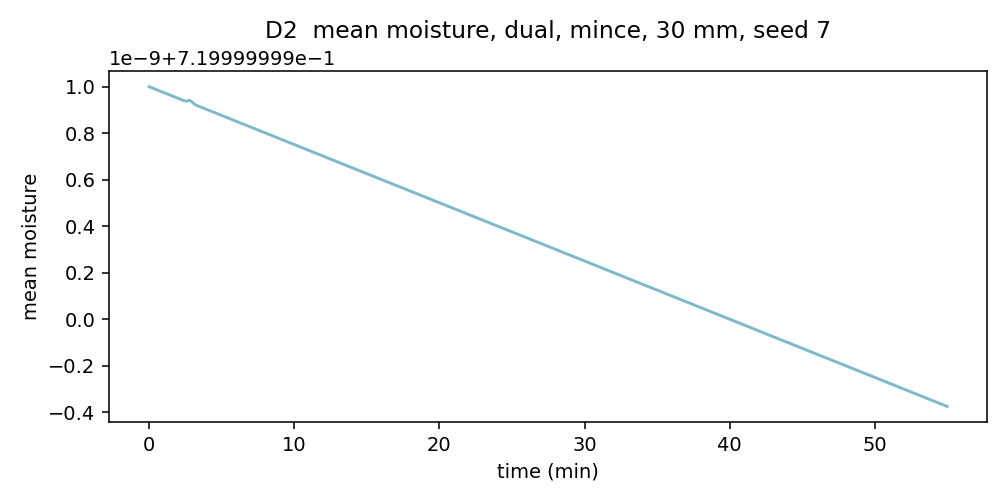
\includegraphics[width=0.86\textwidth]{D2_moisture.png}
\caption{D2。种子 7、肉糜、30 mm、对偶的平均含水。只有这一条，没有三模式。}
\end{figure}

\subsection{D3 致死进度与褐变}
\paragraph{对象}
同一条温度史上 $\alpha_m$ 与 $\alpha_b$ 的分歧。

\paragraph{坐标与应读出的关系}
横轴时间，纵轴进度。两条曲线。

\paragraph{与方程的对应}
核的 $\alpha_m$ 在冷点上积分，$\alpha_b$ 只在表面超过 $110^\circ\mathrm{C}$ 且含水低于 $0.55$ 时增长。

\paragraph{来源}
种子 7 的两条进度已经导出，见 D3。

\paragraph{该图位允许支持的句子}
可以写：终点 $\alpha_m=1$ 不能代替停机时刻的 $\alpha_m$。种子 7 在 1680 s 停机时 $\alpha_m$ 约 $0.755$。褐变在这条轨迹上留在零附近。

\begin{figure}[ht]
\centering
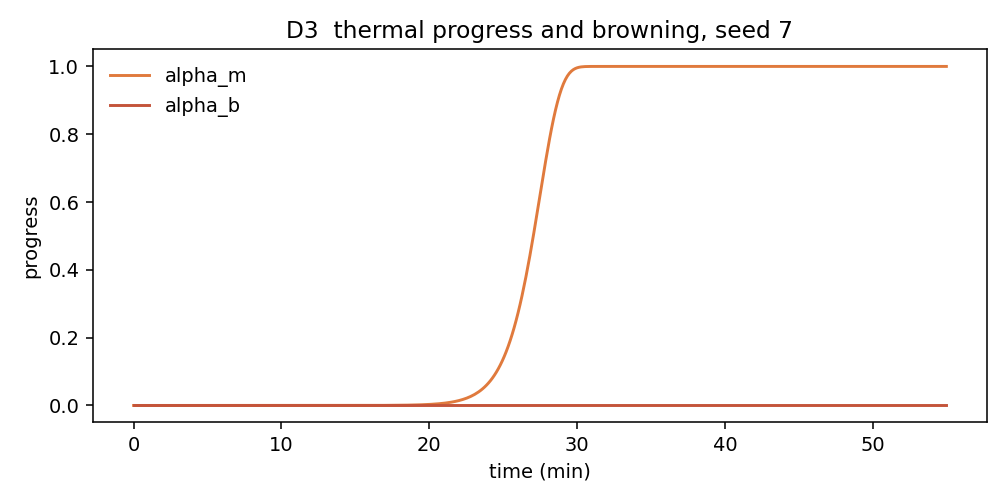
\includegraphics[width=0.86\textwidth]{D3_progress.png}
\caption{D3。同一条种子 7 轨迹上的热力进度和表面褐变。褐变几乎不离开零。}
\end{figure}

\paragraph{该图位不能支持的句子}
不能把该分歧写成美拉德动力学参数已经辨识。

\subsection{D4 结壳与内部热阻}
\paragraph{对象}
结壳变量 $S$ 与内部热阻随时间的联合轨迹。

\paragraph{坐标与应读出的关系}
横轴时间，左轴 $S$，右轴 $R_{\mathrm{int}}$。

\paragraph{与方程的对应}
规格中的反馈见式 \eqref{eq:structure}。核的 $S$ 不改导热。

\paragraph{来源}
没有 $R_{\mathrm{int}}(t)$ 列。不绘制曲线。

\paragraph{该图位允许支持的句子}
可以写：$S$ 只进入参照 $r_{\mathrm{proxy}}$。

\paragraph{该图位不能支持的句子}
不能把参照里的 $2.5S$ 读成导热已经下降。

\subsection{D5 终止时的空间温度}
\paragraph{对象}
停机时刻沿厚度的温度，用来看冷点落在哪一个控制体。

\paragraph{坐标与应读出的关系}
横轴控制体下标或深度，纵轴温度。

\paragraph{与方程的对应}
冷点在核里是最低温度的值，日志不写其下标。

\paragraph{来源}
没有空间分布的导出图。不绘制曲线。

\paragraph{该图位允许支持的句子}
可以写：档 1 与档 2 会改变最低温度的位置，但该位置没有进入摘要。

\paragraph{该图位不能支持的句子}
不能用一条轨迹的冷点数值代替空间曲线。

\subsection{D6 热阻方差}
\paragraph{对象}
探针之后方差是否下降，以及下降的倍数。

\paragraph{坐标与应读出的关系}
横轴时间或脉冲编号，纵轴方差。规格中的纵轴写过 $\log\det\Sigma$；本次只有标量方差。

\paragraph{与方程的对应}
种子 7 在 192 s 从 $0.64$ 降到 $0.224$，比值等于 $0.35$。

\paragraph{来源}
同一条对偶轨迹。不是 P0、P1、P2、P4 的比较。

\paragraph{该图位允许支持的句子}
可以写：下降来自规则中的乘子，而且只在更接近真值参照时发生。

\paragraph{该图位不能支持的句子}
不能把 $0.224$ 写成 Fisher 信息的特征值，也不能写成四个探针的信息增益排序。

\subsection{D7 厚度与进度误差}
\paragraph{对象}
三种厚度上四种策略的进度误差。

\paragraph{坐标与应读出的关系}
横轴厚度 15、30、50 mm，纵轴 $e_\alpha$。每个厚度四个策略。

\paragraph{与方程的对应}
交叉表：15 mm 对偶中位 $-0.417$、无探针 $-0.367$；30 mm 对偶 $-0.080$、无探针 $-0.527$；50 mm 对偶 $-0.598$、无探针 $-0.627$。每格 1620 条。

\paragraph{来源}
S1 日志。图已画出。

\paragraph{该图位允许支持的句子}
可以写：探针的可见差别集中在 30 mm。薄件没有优势。厚件两者都停在设计线之下。

\paragraph{该图位不能支持的句子}
不能把三档的总体中位数 $-0.313$ 写成每一档都改善。

\subsection{D8 含水与厚度的信息增益}
\paragraph{对象}
信息增益 $G$ 在初含水与厚度平面上的等高线。

\paragraph{坐标与应读出的关系}
横轴厚度，纵轴初含水，等高线为 $G$。

\paragraph{与方程的对应}
规格要求这张等高线。核没有计算 $G$。

\paragraph{来源}
图位没有日志，不绘制等高线。

\paragraph{该图位允许支持的句子}
可以写：初含水三档没有改变策略排序的方向，厚度仍是主因子。这是交叉表的结论，不是 $G$ 的等高线。

\paragraph{该图位不能支持的句子}
不能把交叉表的 $e_\alpha$ 填进等高线冒充信息增益。

\subsection{D9 三条路径的增益}
\paragraph{对象}
蒸汽干预增加后，路径 A、B、C 对冷点或表面品质的贡献随厚度变化。

\paragraph{坐标与应读出的关系}
横轴厚度，纵轴路径增益。三条曲线。

\paragraph{与方程的对应}
式 \eqref{eq:path}。增益没有沿后验样本计算。

\paragraph{来源}
图位没有日志，不绘制曲线。

\paragraph{该图位允许支持的句子}
可以写：符号由结构方程指定，数值留空。

\paragraph{该图位不能支持的句子}
不能把对偶与无探针的中位差写成路径 A 的增益。

\subsection{D10 四策略的进度误差}
\paragraph{对象}
开环、腔温比例、无探针、对偶的 $e_\alpha$ 分布。这是主图。

\paragraph{坐标与应读出的关系}
横轴策略，纵轴 $e_\alpha$。零线是设计线。每个策略 4860 条。

\paragraph{与方程的对应}
总体中位：开环 $-0.843$，腔温比例 $+0.150$，无探针 $-0.467$，对偶 $-0.313$。提前比例 $0.667$、$0.222$、$0.944$、$0.902$。

\paragraph{来源}
S1 日志。图已画出。

\paragraph{该图位允许支持的句子}
可以写：腔温比例的质量堆在 $+0.15$，是进度饱和，不是更准的停止。

\paragraph{该图位不能支持的句子}
不能在没有本图时单独用能量下结论。能量表是 D11 的位置，次要指标。

\subsection{D11 能量与停止时刻}
\paragraph{对象}
四种策略的能量中位数和停止时刻中位数。

\paragraph{坐标与应读出的关系}
横轴策略，纵轴能量或时间。能量单位是加热指令乘以记录间隔，不是电度。

\paragraph{与方程的对应}
总体能量中位：开环 1170，腔温比例 3310，无探针 1655，对偶 1730。停止时刻中位 1170、3300、1540、1641 s。

\paragraph{来源}
S1 摘要的中位数，见 D11。D10 在场时这些数才可以引用。

\paragraph{该图位允许支持的句子}
可以写：开环的停止时刻与菜单时间重合。腔温比例的能量高是因为不停机。

\begin{figure}[ht]
\centering
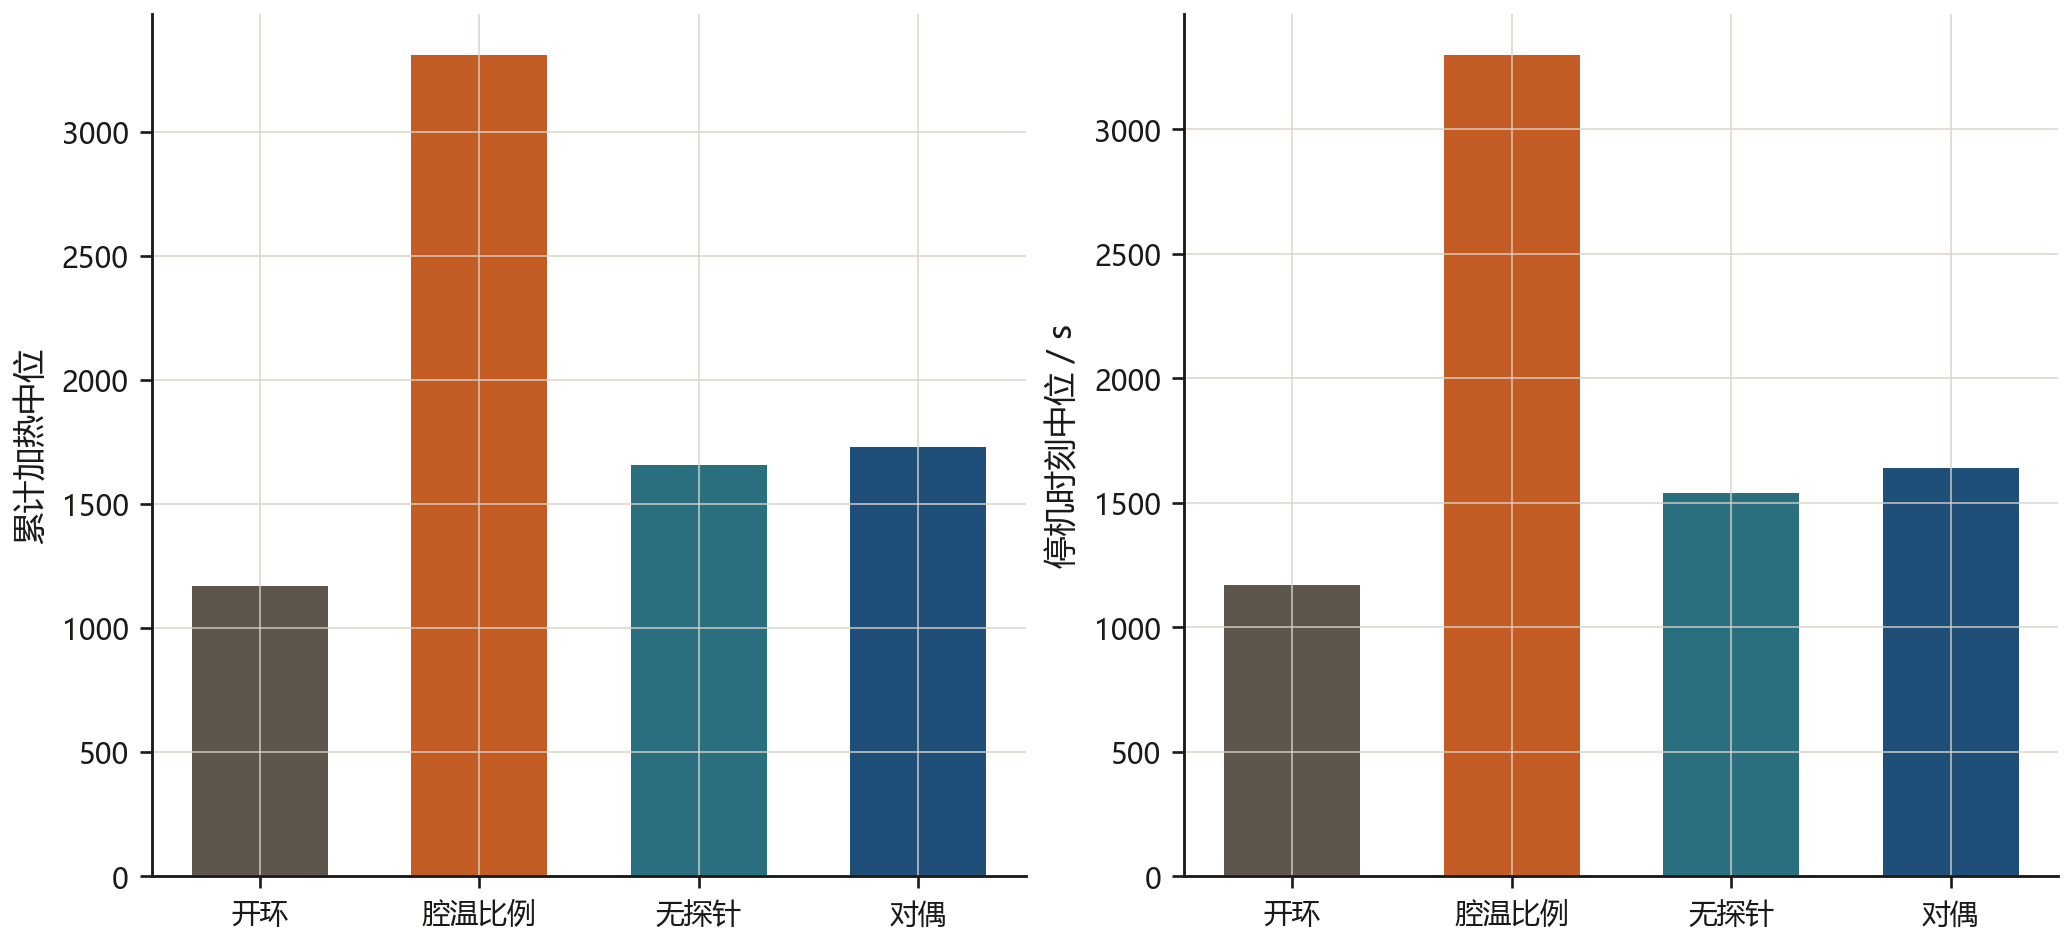
\includegraphics[width=0.92\textwidth]{D11_energy_stop.png}
\caption{D11。四个策略各 4860 行的能量中位数和停止时刻中位数。能量是加热指令乘以记录间隔 10 s。}
\end{figure}

\paragraph{该图位不能支持的句子}
不能把能量低写成策略更安全。厚件开环能量低，同时 $e_\alpha$ 为 $-0.850$。

\subsection{D12 温度均匀性}
\paragraph{对象}
停机时温度场的离散度 $U_T$。

\paragraph{坐标与应读出的关系}
横轴策略，纵轴 $\sigma_T$ 或极差。

\paragraph{与方程的对应}
决策状态里有 $\sigma_T$。S1 的 19440 行没有这一列。S2 在停机时刻记下标准差，只覆盖 30 mm 肉糜。

\paragraph{来源}
S2 摘要的 \texttt{t\_std} 列。没有四策略对照图。

\paragraph{该图位允许支持的句子}
可以写：均匀性仍是规格中的评分项。S1 主表没有用它。S2 只在一条设定上留下了这个数。

\paragraph{该图位不能支持的句子}
不能用冷点与表面的一条温差代替场的标准差分布，也不能把 S2 的一档写成四种策略的均匀性图。

\subsection{D13 质量通道消融}
\paragraph{对象}
有无质量通道时冷点误差的差别。

\paragraph{坐标与应读出的关系}
横轴是通道开关，纵轴 $e_T$。

\paragraph{与方程的对应}
规格中的消融。核的含水是模型状态，不是独立的质量传感器通道。

\paragraph{来源}
图位没有日志，不绘制曲线。

\paragraph{该图位允许支持的句子}
可以写：消融要求两次只差一个通道的运行。本次没有。

\paragraph{该图位不能支持的句子}
不能把带含水的核与一个假想无含水核的差别写成已经测到。

\subsection{D14 热像消融}
\paragraph{对象}
有无热像时冷点误差的差别。

\paragraph{坐标与应读出的关系}
横轴通道开关，纵轴 $e_T$。

\paragraph{与方程的对应}
式 \eqref{eq:ir}。战役没有热像通道。

\paragraph{来源}
图位没有日志，不绘制曲线。

\paragraph{该图位允许支持的句子}
可以写：表面温度通道是带噪接触读数，噪声 $0.4^\circ\mathrm{C}$。

\paragraph{该图位不能支持的句子}
不能把该噪声写成热像消融的结果。

\subsection{D15 遮挡与探针有效率}
\paragraph{对象}
热像被蒸汽遮挡的时长与探针有效率。

\paragraph{坐标与应读出的关系}
横轴遮挡时长，纵轴有效率。

\paragraph{与方程的对应}
有效的定义是探针后协方差降到预测的一定比例。核没有这个计数器。

\paragraph{来源}
S2 的表面保持，见 D15。保持的是表面温度读数，不是热像遮挡。核没有有效率计数器。

\paragraph{该图位允许支持的句子}
可以写：在 30 mm 肉糜、对偶、40 个种子上，保持 60 s 后中位数从 \(-0.112\) 变到 \(-0.067\)，仍为负。终点方差仍是 0.224。

\paragraph{该图位不能支持的句子}
不能把种子 7 的方差下降写成遮挡时长为零时的有效率。也不能把表面读数保持写成热像已经被遮挡。

\begin{figure}[ht]
\centering
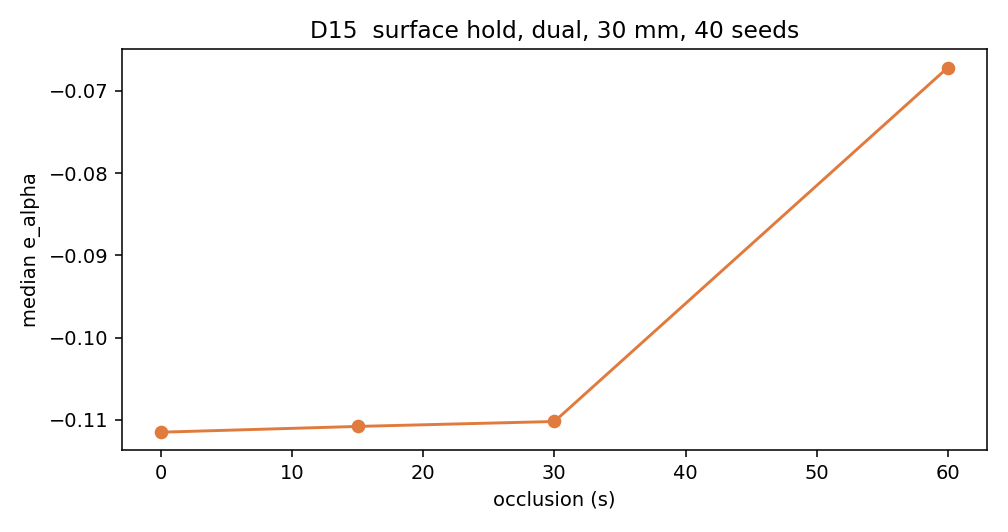
\includegraphics[width=0.86\textwidth]{D15_occlusion.png}
\caption{D15。表面读数保持初值的时间与中位停机误差。同一张图也放在第 \ref{ch:sim} 章。}
\end{figure}

\subsection{D16 噪声倍数}
\paragraph{对象}
观测噪声放大倍数与 $e_\alpha$ 的关系。

\paragraph{坐标与应读出的关系}
横轴噪声倍数，纵轴进度误差。

\paragraph{与方程的对应}
核的噪声幅度固定。没有倍数扫描。

\paragraph{来源}
图位没有日志，不绘制曲线。

\paragraph{该图位允许支持的句子}
可以写：噪声用正弦散列，换倍数会改变散列幅度，但本次没有那次运行。

\paragraph{该图位不能支持的句子}
不能把 30 个种子的散布写成噪声倍数扫描。种子散布是初值和参数格子上的样本。

\subsection{D17 算子种类}
\paragraph{对象}
FNO 与 DeepONet 在干预位移上的误差。

\paragraph{坐标与应读出的关系}
横轴算子种类，纵轴位移误差。

\paragraph{与方程的对应}
式 \eqref{eq:op}。两个算子都没有训练。

\paragraph{来源}
图位没有日志，不绘制柱。不宣布胜者。

\paragraph{该图位允许支持的句子}
可以写：比较要在含干预的教师集上做，而且教师集不能进入主表。

\paragraph{该图位不能支持的句子}
不能根据文献中别人的误差选择一个算子作为本文结果。

\subsection{D18 残差界与回退次数}
\paragraph{对象}
残差上界与回退次数。

\paragraph{坐标与应读出的关系}
横轴 $r_{\max}$，纵轴回退次数。

\paragraph{与方程的对应}
式 \eqref{eq:bnp}。没有残差模块。

\paragraph{来源}
图位没有日志，不绘制曲线。

\paragraph{该图位允许支持的句子}
可以写：回退是规格中的安全行为，不是本次计数。

\paragraph{该图位不能支持的句子}
不能把热阻不更新的那些样本计成回退。不更新是因为没有更接近参照，不是因为残差越界。

\subsection{D19 请求加热与投影加热}
\paragraph{对象}
贴近屏障时，请求与投影后的指令分开。

\paragraph{坐标与应读出的关系}
横轴时间，两条加热指令。

\paragraph{与方程的对应}
核的削减在 $T_h>230^\circ\mathrm{C}$ 时动作。平衡点 $196.5^\circ\mathrm{C}$。

\paragraph{来源}
种子 7 的请求和指令，见 D19。两条曲线在这条轨迹上重合。

\paragraph{该图位允许支持的句子}
可以写：这条轨迹上请求与指令重合，因为加热器没有越过 \(230^\circ\mathrm{C}\)。

\begin{figure}[ht]
\centering
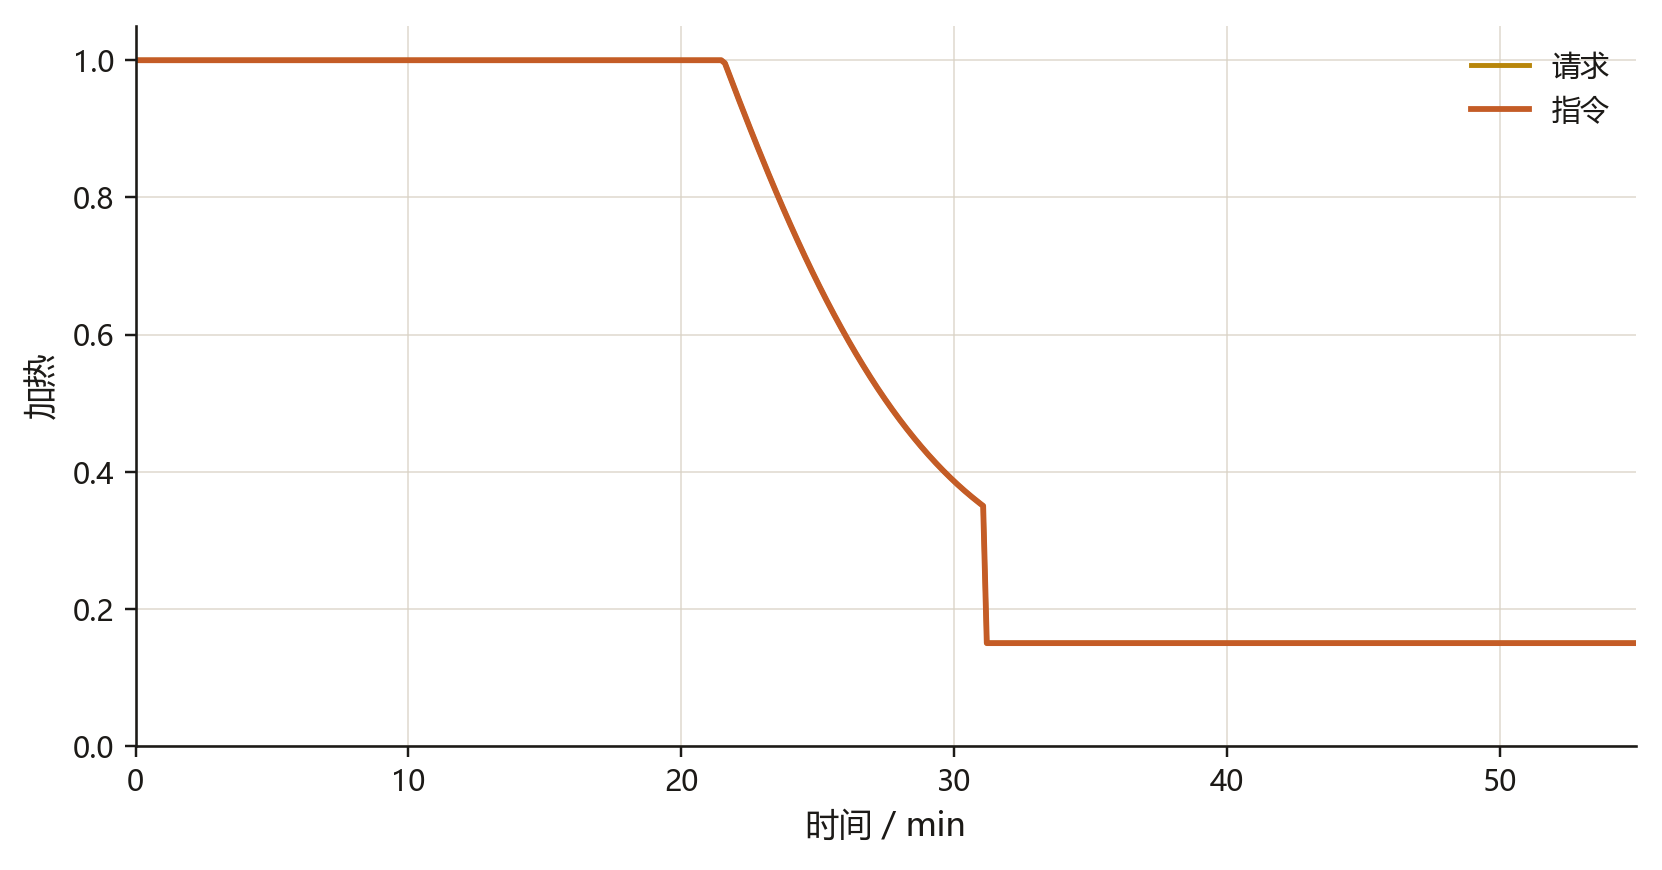
\includegraphics[width=0.86\textwidth]{D19_projection.png}
\caption{D19。种子 7 的加热请求与加热指令。两条线重合。削减阈值没有被碰到。}
\end{figure}

\paragraph{该图位不能支持的句子}
不能把断言函数在 $210^\circ\mathrm{C}$ 的剪切画进 S1 轨迹。

\subsection{D20 去掉屏障的消融}
\paragraph{对象}
有无测量隔离时的越界次数。

\paragraph{坐标与应读出的关系}
横轴是否隔离，纵轴越界次数。

\paragraph{与方程的对应}
命题 \ref{prop:shield}。越界计数器没有在战役里运行。

\paragraph{来源}
图位没有日志，不绘制柱。

\paragraph{该图位允许支持的句子}
可以写：隔离的含义是投影不读后验。本次投影没有改变指令。

\paragraph{该图位不能支持的句子}
不能把能量中位数的差别写成越界次数。

\subsection{D21 同构与异构}
\paragraph{对象}
真值与估计器同构时的误差，对照异构时的误差。

\paragraph{坐标与应读出的关系}
横轴同构或异构，纵轴 $e_\alpha$。

\paragraph{与方程的对应}
同构结果只做数值自检，不进入主表，也不进入摘要句。

\paragraph{来源}
异构配对没有运行。不绘制柱。

\paragraph{该图位允许支持的句子}
可以写：本次全部数字的主语是同一个工程核。

\paragraph{该图位不能支持的句子}
不能把 4860 条写成异构感知误差。

\subsection{D22 厚件上的区间宽度}
\paragraph{对象}
50 mm 上进度或剩余时间的区间宽度，用来拒绝单点剩余时间。

\paragraph{坐标与应读出的关系}
横轴样本，纵轴区间宽度。

\paragraph{与方程的对应}
规格：信息上界低于停机所需熵减时输出区间。核没有区间输出。

\paragraph{来源}
图位没有日志，不绘制曲线。50 mm 的对偶与无探针都提前停止，提前比例都是 1。

\paragraph{该图位允许支持的句子}
可以写：厚件上固定窗没有把中位误差拉到零附近。

\paragraph{该图位不能支持的句子}
不能把提前比例为 1 写成已经拒绝了单点时间。界面没有这个输出。

\subsection{D23 种子与停止时刻}
\paragraph{对象}
停止时刻对种子的散布，用来核对可复现性。

\paragraph{坐标与应读出的关系}
横轴种子编号，纵轴停止时刻。

\paragraph{与方程的对应}
种子进入正弦散列的相位。同一代码重复运行得到同一轨迹。

\paragraph{来源}
15 mm、肉糜、初温 \(5^\circ\mathrm{C}\)、含水 0.72、导热缺损这一格的四个策略，见 D23。

\paragraph{该图位允许支持的句子}
可以写：开环停止时刻不随种子变化，因为菜单时间只依赖厚度。对偶在这一格上随种子分成两簇停止时刻。

\begin{figure}[ht]
\centering
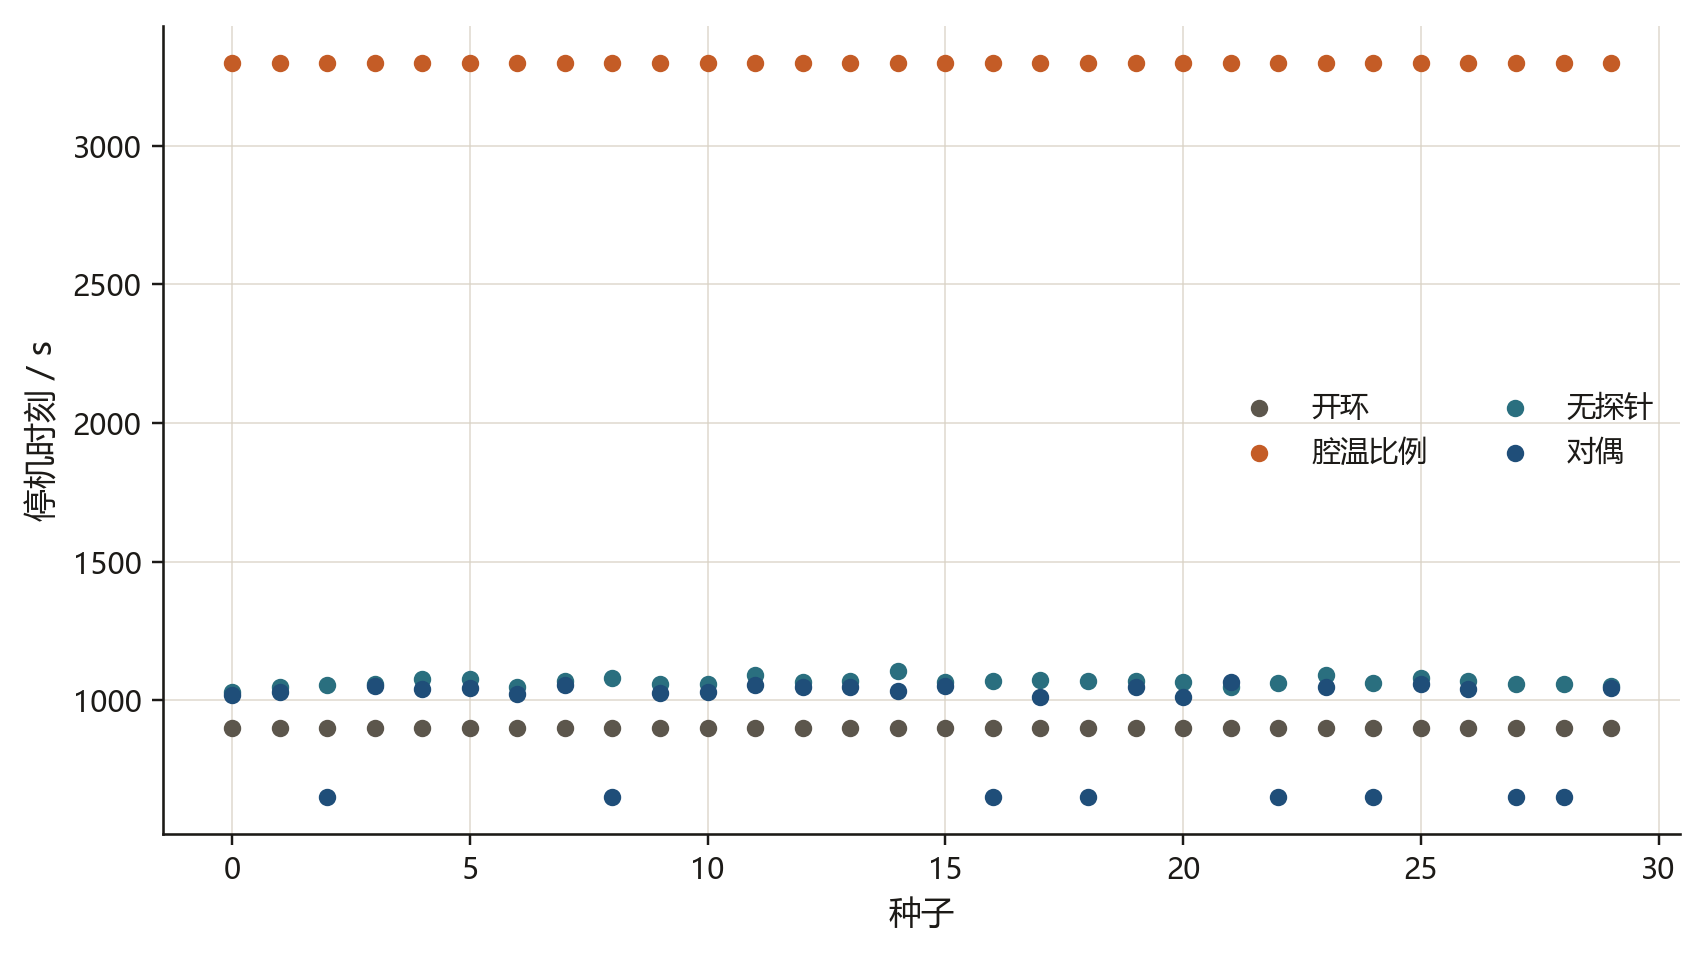
\includegraphics[width=0.86\textwidth]{D23_seed_stop.png}
\caption{D23。一个 15 mm 格子里，停止时刻对种子编号。开环是一条水平线。对偶分成两簇。}
\end{figure}

\paragraph{该图位不能支持的句子}
不能把散点的宽度写成物理重复实验的不确定度。

\subsection{D24 降级级别与停留时间}
\paragraph{对象}
五级降级各自的停留时间。

\paragraph{坐标与应读出的关系}
横轴级别，纵轴时间。

\paragraph{与方程的对应}
第 \ref{ch:safe} 章。战役没有在这些级别之间切换。

\paragraph{来源}
图位没有日志，不绘制柱。

\paragraph{该图位允许支持的句子}
可以写：模式整数里的保持不是通道失效。

\paragraph{该图位不能支持的句子}
不能把停机后的低功率时长写成第 4 级停留时间。

\subsection{D25 原型与策略}
\paragraph{对象}
肉糜、土豆、面团在四种策略上的中位 $e_\alpha$。

\paragraph{坐标与应读出的关系}
横轴原型，分组为策略。每格 1620 条。

\paragraph{与方程的对应}
三个原型的中位几乎相同。核里原型只改活度尺度，而且在初含水格子上活度都饱和。

\paragraph{来源}
S1 日志。图已画出。

\paragraph{该图位允许支持的句子}
可以写：排序不依赖这三个食材标签。

\paragraph{该图位不能支持的句子}
不能写成蛋白与淀粉的反应差异已经检验。

\subsection{D26 冷点离开几何中心的距离}
\paragraph{对象}
非均质档位与冷点到几何中心的距离，并对照 T1 与 T2。

\paragraph{坐标与应读出的关系}
横轴非均质档，纵轴距离。

\paragraph{与方程的对应}
T2 未运行。S2 在停机时刻记下冷点所在的控制体下标，只覆盖 30 mm 肉糜这一档，没有画成距离分布。

\paragraph{来源}
S2 摘要的 \texttt{cold\_index\_stop} 列。没有 T1 对 T2 的图。

\paragraph{该图位允许支持的句子}
可以写：档 2 把下标 5 的导热乘 $0.45$。这是机制。S2 只说明这一档记下了下标，不是距离的分布。

\paragraph{该图位不能支持的句子}
不能用一个控制体的位置代替冷点位移的分布。

\subsection{D27 含水偏差与信息增益}
\paragraph{对象}
先验含水偏差是否把探针的信息增益吞掉。

\paragraph{坐标与应读出的关系}
横轴含水偏差，纵轴 $G_{\mathrm{real}}$。

\paragraph{与方程的对应}
没有 $G$ 的计算。初含水三档的交叉表没有改变厚度这个主因子。

\paragraph{来源}
图位没有信息增益日志，不绘制曲线。

\paragraph{该图位允许支持的句子}
可以写：含水档是因子，不是信息增益的横轴。

\paragraph{该图位不能支持的句子}
不能把 $e_\alpha$ 对含水的弱变化写成 $G$ 已被先验误差吞掉。

\subsection{D28 噪声倍数与探针有效率}
\paragraph{对象}
S2 中噪声倍数对探针有效率的影响。

\paragraph{坐标与应读出的关系}
横轴噪声倍数，纵轴有效率。

\paragraph{与方程的对应}
S2 没有做噪声倍数。对偶的更新不乘这个倍数，所以没有有效率可报。

\paragraph{来源}
没有倍数轴，不绘制曲线。

\paragraph{该图位允许支持的句子}
可以写：有效率的分母尚未定义在计数器里。S2 已经运行的是表面保持、质量通道、脂肪层和一次开门。

\paragraph{该图位不能支持的句子}
不能用 S2 的表面保持代替噪声倍数。

\subsection{D29 遮挡与区间宽度}
\paragraph{对象}
遮挡时长与剩余时间区间宽度。

\paragraph{坐标与应读出的关系}
横轴遮挡时长，纵轴区间宽度。

\paragraph{与方程的对应}
没有遮挡注入，没有区间输出。

\paragraph{来源}
图位没有日志，不绘制曲线。

\paragraph{该图位允许支持的句子}
可以写：拒绝单点时间是规格中的界面行为。

\paragraph{该图位不能支持的句子}
不能把方差 $0.224$ 换算成区间宽度。

\subsection{D30 脂肪层与路径 C}
\paragraph{对象}
脂肪层开关打开时，慢路径 C 是否出现。

\paragraph{坐标与应读出的关系}
横轴脂肪层开关，纵轴路径 C 的增益。

\paragraph{与方程的对应}
路径 C 要求结壳改变导热。核的结壳不改导热。档 2 只改一个控制体的初始导热。

\paragraph{来源}
图位没有路径增益，不绘制柱。

\paragraph{该图位允许支持的句子}
可以写：档 2 的额外串联热阻约占 $7.6\%$。这是几何算术，不是路径 C 的干预效应。

\paragraph{该图位不能支持的句子}
不能把厚件仍然提前写成脂肪层已经检验了慢路径。

\subsection{D31 活化能扫描}
\paragraph{对象}
$E_a$ 改变时 $\alpha_m$ 的变化。

\paragraph{坐标与应读出的关系}
横轴活化能，纵轴进度。

\paragraph{与方程的对应}
式 \eqref{eq:kinetics}。核的 $F$ 使用固定的 $z=10$ K 和除数 2，没有活化能扫描。

\paragraph{来源}
图位没有日志，不绘制曲线。

\paragraph{该图位允许支持的句子}
可以写：设计线 $F\approx 3.79$ min 依赖除数 2。换除数会移动零点。

\paragraph{该图位不能支持的句子}
不能把除数 2 写成某一微生物的 $D$ 值。

\subsection{D32 集合规模}
\paragraph{对象}
32 个成员与 128 个成员的方差比。

\paragraph{坐标与应读出的关系}
横轴集合规模，纵轴方差比。

\paragraph{与方程的对应}
规格中的在线集合与离线对照。两者都没有运行。

\paragraph{来源}
图位没有日志，不绘制柱。

\paragraph{该图位允许支持的句子}
可以写：本次方差是标量规则的乘子，不是集合样本方差。

\paragraph{该图位不能支持的句子}
不能把 $0.35$ 写成 128 个成员相对 32 个成员的方差比。

\subsection{D33 风速与换热系数}
\paragraph{对象}
T3 边界库中风速与 $h$ 的关系。

\paragraph{坐标与应读出的关系}
横轴风速，纵轴 $h$。

\paragraph{与方程的对应}
核使用 $h=12+55\,u_{\mathrm{fan}}$。风机指令不是以 m/s 记录的风速。

\paragraph{来源}
T3 未运行。不把线性式画成实测边界库。

\paragraph{该图位允许支持的句子}
可以写：探针段风机 $1.3$ 时 $h=83.5$，30 mm 的 Biot 数约 $3.7$。这是尺度算术。

\paragraph{该图位不能支持的句子}
不能把该直线写成腔体混合实验的拟合。

\subsection{D34 停止时刻差}
\paragraph{对象}
同一组合上对偶相对无探针的停止时刻差，对种子的分布。

\paragraph{坐标与应读出的关系}
横轴种子分位，纵轴停止时刻差。

\paragraph{与方程的对应}
交叉表给出的是中位数，不是这条差的分位曲线。30 mm 上停止时刻中位从 1540 s 到 1641 s。

\paragraph{来源}
差的分布没有单独导出。不另画未导出的曲线。

\paragraph{该图位允许支持的句子}
可以写：30 mm 上对偶停得更晚，与中位误差从 $-0.527$ 到 $-0.080$ 同方向。

\paragraph{该图位不能支持的句子}
不能把 101 s 的中位差写成每一个种子都晚停 101 s。

\subsection{D35 扩充标记}
\paragraph{对象}
教师扩充样本是否进入主表。

\paragraph{坐标与应读出的关系}
横轴扩充标记，纵轴干预误差。

\paragraph{与方程的对应}
全部战役行的扩充标记为假，来源字段为 simulation。

\paragraph{来源}
没有教师集，没有干预误差。不绘制柱。

\paragraph{该图位允许支持的句子}
可以写：主表的分母是 4860 个未扩充的组合。

\paragraph{该图位不能支持的句子}
不能把扩充样本的误差写进摘要。样本不存在。

\subsection{D36 来源字段}
\paragraph{对象}
参数轴上每一项来自 DOI、文献区间还是仿真。

\paragraph{坐标与应读出的关系}
横轴参数，纵轴来源类别。三类互斥。

\paragraph{与方程的对应}
允许的值只有 \texttt{doi:10.5281/zenodo.21671925}、\texttt{literature-interval}、\texttt{simulation}。

\paragraph{来源}
等温线参数可以标 DOI。核的导热、潜热系数和反应除数是设定。战役行的来源字段全部是 simulation。

\paragraph{该图位允许支持的句子}
可以写：第三个值不出现在摘要的验证句里。

\paragraph{该图位不能支持的句子}
不能把土豆的 $X_m$ 标到来源为仿真的肉糜活度上。

\section{实施例图}

实施例图画在同一腔体上。只标模型用到的量。安全侧与食品侧分开。没有采样的感知点不标成已经记录的通道。

\subsection{E1 腔体截面}
\paragraph{对象}
加热、蒸汽、风、排汽在腔体截面上的位置。只标模型用到的量。

\paragraph{坐标与应读出的关系}
截面。标 $u$、$u_{\mathrm{st}}$、$u_{\mathrm{fan}}$ 和排汽对腔体湿度的影响。不标没有进入方程的零件。

\paragraph{与方程的对应}
界面通量 $h(T_\infty-T_0)+q_{\mathrm{lat}}+7000\,u$。$h=12+55\,u_{\mathrm{fan}}$，$T_\infty=90+95\,u$。

\paragraph{来源}
实施例图。角系数和 $T^4$ 不在核里，图上不标成已经使用的传感器。

\paragraph{该图位允许支持的句子}
可以写：排汽在规格里降低腔体湿度，使蒸发恢复。核用蒸汽指令的开关代替了这一路。

\paragraph{该图位不能支持的句子}
不能把截面图画成流场已经求解。T3 未运行。

\subsection{E2 食品侧观测}
\paragraph{对象}
质量与热像视场在食品侧的位置。穿刺探针只出现在对照侧。

\paragraph{坐标与应读出的关系}
食品与腔体的界面。主观测是表面温度和平均含水的带噪读数。穿刺不进入主观测向量。

\paragraph{与方程的对应}
第 1 章：穿刺能降低停机不确定度，但改变局部场，而且不刺中冷点时不代表 $\operatorname{ess\,inf} T$。

\paragraph{来源}
实施例图。质量和热像本次没有采样。

\paragraph{该图位允许支持的句子}
可以写：可重构性不依赖穿刺通道。

\paragraph{该图位不能支持的句子}
不能把种子 7 的冷点曲线画成穿刺探针的读数。

\subsection{E3 安全侧感知点}
\paragraph{对象}
漏电、水位、管温、门、腔压。这些点与 E2 分开。

\paragraph{坐标与应读出的关系}
安全侧。每一点只与阈值比较。

\paragraph{与方程的对应}
第 \ref{ch:safe} 章。本次只有加热器温度进入削减逻辑，而且没有越过阈值。

\paragraph{来源}
实施例图。

\paragraph{该图位允许支持的句子}
可以写：硬测量不进入品质网络的特征。

\paragraph{该图位不能支持的句子}
不能把这些感知点画成已经有采样列。

\subsection{E4 P4 在执行器上的时序}
\paragraph{对象}
与 M18 相同的两段时序，画在执行器指令上。

\paragraph{坐标与应读出的关系}
蒸汽与风机的阶跃。已运行窗 $[150,190)$ s。

\paragraph{与方程的对应}
命题 \ref{prop:pulse} 与附录的离散格式。

\paragraph{来源}
实施例图，与 M18 使用同一组常数。

\paragraph{该图位允许支持的句子}
可以写：170 s 是两段的分界，190 s 是更新时刻。

\paragraph{该图位不能支持的句子}
不能把时序改成随厚度变化的最优波形。厚度没有进入窗的起止时刻。

\subsection{E5 界面上的路径数值}
\paragraph{对象}
路径 A 与路径 B 在界面上的数值。定义与 D9 相同。

\paragraph{坐标与应读出的关系}
两个数或两条箭。数值留空，直到 D9 有日志。

\paragraph{与方程的对应}
式 \eqref{eq:path}。

\paragraph{来源}
实施例图。与 D9 一样没有路径增益。

\paragraph{该图位允许支持的句子}
可以写：界面是路径分叉的位置。

\paragraph{该图位不能支持的句子}
不能填上对偶与无探针的能量差。

\subsection{E6 投影前后的加热指令}
\paragraph{对象}
投影前的请求与投影后的指令。定义与 D19 相同。

\paragraph{坐标与应读出的关系}
两条时间序列。本次二者重合。

\paragraph{与方程的对应}
削减公式与命题 \ref{prop:shield} 的断言函数是两段代码。

\paragraph{来源}
实施例图。不画未发生的分离。

\paragraph{该图位允许支持的句子}
可以写：重合是因为加热器平衡低于两个阈值。

\paragraph{该图位不能支持的句子}
不能把 $0.25$ 的断言剪切标成战役指令。

\subsection{E7 降级后的区间显示}
\paragraph{对象}
降级后面板上的区间，而不是单点分钟数。

\paragraph{坐标与应读出的关系}
一个区间。端点由进度分位换算。分位不存在时面板不应出现数字。

\paragraph{与方程的对应}
第 \ref{ch:safe} 章与 D22。核没有区间输出。

\paragraph{来源}
实施例图。不填一个剩余分钟数。

\paragraph{该图位允许支持的句子}
可以写：50 mm 上提前比例为 1，说明点估计停机在该厚度上没有停在设计线。

\paragraph{该图位不能支持的句子}
不能把中位停止时刻 3300 s 写成剩余时间的预测。

\subsection{E8 数据文件与页面四块}
\paragraph{对象}
下载文件的列与页面四块的对应。列名与第 \ref{ch:demo} 章相同。

\paragraph{坐标与应读出的关系}
四块：轨迹、路径、投影、下载。列包括时间、表面温度、冷点、估计冷点、含水、进度、方差、加热、加热请求、蒸汽、模式。

\paragraph{与方程的对应}
第 \ref{ch:demo} 章。战役记录还含风机、加热器温度和真值参照。浏览器副本的列集合若更窄，不进入主表。

\paragraph{来源}
实施例图。

\paragraph{该图位允许支持的句子}
可以写：导出由数值核序列化。界面不另写差分。

\paragraph{该图位不能支持的句子}
不能把浏览器副本的中位数写进交叉表。


88 个图位的文字说明计入正文。每条说明包含对象、坐标、方程或协议、来源、允许支持的句子和不能支持的句子。仅有图号而没有这些句子的位置，不计入技术内容。

没有日志的数据图位保持为坐标。把一条种子轨迹填进这些坐标，会把单条样本写成该图位所要求的对照。本章不这样做。
